\documentclass[12pt]{article}

% -------------------------------------------------------------------
% PACKAGES
% -------------------------------------------------------------------
\usepackage[T1]{fontenc}
\usepackage[utf8]{inputenc}
\usepackage[english]{babel}
\usepackage[margin=1in]{geometry}
\usepackage{graphicx}
\usepackage{caption}
\usepackage{amsmath, amssymb}
\usepackage{tikz}
\usetikzlibrary{arrows.meta, positioning}

% -------------------------------------------------------------------
% TITLE & AUTHOR
% -------------------------------------------------------------------
\title{RSA Key Management and Security Analysis \\
       \large Methods, Correctness, and Conceptual Framework}
\author{Your Name}
\date{\today}

% -------------------------------------------------------------------
% DOCUMENT
% -------------------------------------------------------------------
\begin{document}

\maketitle

\tableofcontents
\clearpage

% -------------------------------------------------------------------
% 1. INTRODUCTION
% ----------------------------------------------------------------

% -------------------------------------------------------------------
% 2. KEY MANAGEMENT
% -------------------------------------------------------------------
\section{Key Management System}
The \emph{key management} logic is encapsulated in a specialized class (e.g., \texttt{RSAKeyManager}), which handles:
\begin{itemize}
    \item Generating a new RSA keypair.
    \item Persisting the keypair (public and private keys) to files.
    \item Storing \emph{metadata}, including creation time, expiration time, and key size.
    \item Checking whether a key has expired and rotating keys if necessary.
\end{itemize}

\subsection{Methods Used}
\begin{enumerate}
    \item \textbf{RSA Key Generation:} 
    A new RSA keypair is generated by calling a method from the core RSA class. The key size can be configured (e.g., 2048 bits for security or smaller for demonstrations).
    
    \item \textbf{Metadata Management:}
    The metadata file (\texttt{JSON} format) stores:
    \begin{itemize}
        \item \texttt{creation\_time}: UTC timestamp of when the key was generated.
        \item \texttt{expiration\_time}: UTC timestamp, computed by adding a specified number of days to the creation time.
        \item \texttt{key\_size}: The integer size in bits (e.g., 2048).
    \end{itemize}

    \item \textbf{Expiration Check:}
    The system compares the current UTC time with the stored \texttt{expiration\_time}. If the key is past its validity period, it is considered invalid and triggers a rotation.

    \item \textbf{Key Rotation:}
    Upon expiration, the old keys are replaced with a fresh keypair. The metadata file is also updated to reflect the new key attributes.
\end{enumerate}

\subsection{Correctness and Robustness}
\begin{itemize}
    \item \textbf{Correct Key Storage:} 
    Correctness is ensured by verifying the presence of both public and private key files before usage. If keys do not exist, the system prompts a regeneration.
    
    \item \textbf{Expiration Safety:}
    Storing the expiration timestamp and enforcing rotation reduces the likelihood of using compromised or aged keys. Once an expired key is detected, the application reliably replaces it.

    \item \textbf{Metadata Integrity:}
    The system expects the metadata file to remain uncorrupted. If it is missing or unreadable, the code defaults to a safe response (considering the key invalid or expired) to avoid potential confusion around unknown or stale keys.
\end{itemize}

\subsection{Conceptual Diagram}

\begin{figure}[h!]
\centering
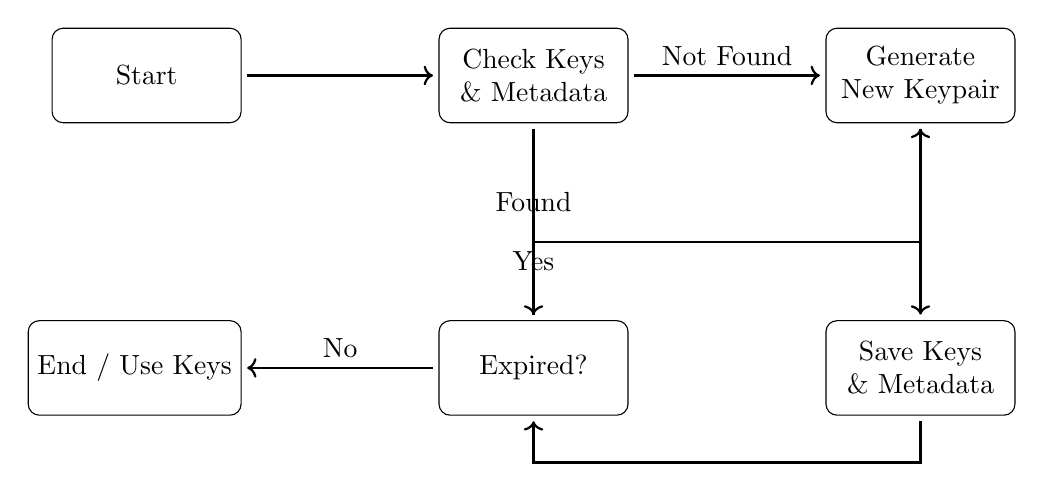
\begin{tikzpicture}[
    node distance=2.5cm, 
    box/.style={rectangle, draw, rounded corners, align=center, minimum width=2.4cm, minimum height=1.2cm},
    arrow/.style={->, thick, shorten >=2pt, shorten <=2pt}
]

% Nodes
\node[box] (start) {Start};
\node[box, right=of start] (check) {Check Keys \\ \& Metadata};
\node[box, right=of check] (generate) {Generate \\ New Keypair};
\node[box, below=of generate] (save) {Save Keys \\ \& Metadata};
\node[box, left=of save] (expire) {Expired?};
\node[box, left=of expire] (end) {End / Use Keys};

% Arrows
\draw[arrow] (start) -- (check);
\draw[arrow] (check) -- node[above]{Not Found} (generate);
\draw[arrow] (check) -- node[above]{Found} (expire);
\draw[arrow] (generate) -- (save);
\draw[arrow] (save) -- ++(0,-1.2) -| (expire);
\draw[arrow] (expire) -- node[above]{Yes} ++(0,1.6) -| (generate);
\draw[arrow] (expire) -- node[above]{No} (end);

\end{tikzpicture}
\caption{Key Management Workflow}
\label{fig:key_management_workflow}
\end{figure}

In Figure~\ref{fig:key_management_workflow}:
\begin{enumerate}
    \item The system begins by checking whether key files and metadata exist.
    \item If missing, new keys are created and saved.
    \item If present, the system evaluates whether the keys have expired.
    \item If expired, the keys are regenerated and saved (rotated).
    \item Otherwise, the keys are ready for normal usage.
\end{enumerate}

% -------------------------------------------------------------------
% 3. Implementation Details
% -------------------------------------------------------------------

\section{Implementation Details}
This section presents a detailed implementation of the RSA cryptosystem in Python, featuring robust key generation, secure padding mechanisms, and timing attack mitigations.

\subsection{Core RSA Class Implementation}
The implementation centers around a primary \texttt{RSA} class that encapsulates all cryptographic operations. The class provides a comprehensive interface for key generation, message padding, encryption, and decryption.

\subsubsection{Key Generation}
The key generation process implements several crucial security features:

\begin{itemize}
    \item \textbf{Secure Prime Generation:} Utilizes the Miller-Rabin primality test with 128 rounds for high confidence in prime number generation:
    \begin{verbatim}
    def is_prime(self, n: int, k: int = 128) -> bool:
        if n == 2 or n == 3:
            return True
        if n < 2 or n % 2 == 0:
            return False
        
        r, d = 0, n - 1
        while d % 2 == 0:
            r += 1
            d //= 2
    \end{verbatim}

    \item \textbf{Cryptographically Secure Random Number Generation:} Employs Python's \texttt{secrets} module instead of the standard \texttt{random} module for generating prime candidates:
    \begin{verbatim}
    def generate_prime(self, bits: int) -> int:
        while True:
            n = secrets.randbits(bits)
            n |= (1 << bits - 1) | 1
            if self.is_prime(n, 128):
                return n
    \end{verbatim}
\end{itemize}

\subsubsection{Message Padding}
The implementation includes PKCS\#1 v1.5 style padding for enhanced security:

\begin{itemize}
    \item \textbf{Padding Implementation:} Follows the format: \texttt{00 || 02 || PS || 00 || M}
    \item \textbf{Random Padding:} Generates non-zero random bytes for the padding string (PS)
    \item \textbf{Length Validation:} Ensures messages don't exceed the maximum length based on key size
\end{itemize}

The padding method includes crucial security checks:
\begin{verbatim}
def pad_message(self, message: Union[str, bytes]) -> int:
    if isinstance(message, str):
        message = message.encode('utf-8')
    
    max_message_length = self.key_size // 8 - 11
    if len(message) > max_message_length:
        raise ValueError(f"Message too long")
        
    padding_length = self.key_size // 8 - len(message) - 3
    padding = b''
    while len(padding) < padding_length:
        byte = secrets.token_bytes(1)
        if byte != b'\x00':
            padding += byte
\end{verbatim}

\subsubsection{Encryption and Decryption}
The core cryptographic operations implement several security measures:

\begin{itemize}
    \item \textbf{Timing Attack Mitigation:} Both encryption and decryption operations include constant-time padding:
    \begin{verbatim}
    start_time = time.time()
    cipher = pow(padded, e, n)
    time.sleep(0.001 - ((time.time() - start_time) % 0.001))
    \end{verbatim}
    
    \item \textbf{Input Validation:} Checks for key availability and appropriate message sizes:
    \begin{verbatim}
    if not self.public_key:
        raise ValueError("No public key available")
        
    if cipher >= n:
        raise ValueError("Ciphertext too large")
    \end{verbatim}
\end{itemize}

\subsection{Performance Analysis}
The implementation includes performance monitoring capabilities:

\begin{itemize}
    \item \textbf{Timing Measurements:} Records encryption and decryption times:
    \begin{verbatim}
    start_time = datetime.now()
    encrypted = rsa.encrypt(message)
    encryption_time = (datetime.now() - 
                      start_time).total_seconds()
    \end{verbatim}
    
    \item \textbf{Key Generation Monitoring:} Tracks the time taken for key generation and primality testing
\end{itemize}

\subsection{Security Considerations}
The implementation addresses several security aspects:

\begin{itemize}
    \item \textbf{Strong Prime Generation:} Uses cryptographically secure random number generation
    \item \textbf{Proper Padding:} Implements PKCS\#1 v1.5 padding scheme
    \item \textbf{Timing Attack Protection:} Implements constant-time operations
    \item \textbf{Input Validation:} Includes comprehensive error checking
\end{itemize}

\subsection{Future Enhancements}
Potential improvements to the current implementation could include:

\begin{itemize}
    \item \textbf{OAEP Padding:} Upgrading to more modern PKCS\#1 v2.0 OAEP padding
    \item \textbf{Additional Side-Channel Protections:} Implementing blinding techniques
    \item \textbf{Performance Optimizations:} Using the Chinese Remainder Theorem for decryption
    \item \textbf{Memory Security:} Implementing secure memory wiping for sensitive values
\end{itemize}

% -------------------------------------------------------------------
% 4. SECURITY ANALYSIS
% -------------------------------------------------------------------
\section{Security Analysis}

\subsection{Naive Factoring of Small RSA Moduli}
\subsubsection{Principle}
One component of the security analysis is to demonstrate the ease of factoring \emph{small} RSA moduli. An RSA modulus \(n\) is simply the product of two primes \(p\) and \(q\). If the key size is extremely small (e.g., 32 or 48 bits total), a brute-force or naive approach that attempts dividing \(n\) by candidate factors up to \(\sqrt{n}\) will succeed quickly.

\subsubsection{Method}
\begin{itemize}
    \item \textbf{Enumerate possible factors:} Start from 3 and increment in steps of 2 (skipping even numbers), testing for divisibility of \(n\).
    \item \textbf{Stop at \(\sqrt{n}\):} If \(p\) is a prime factor, it cannot exceed \(\sqrt{n}\). Thus, searching beyond \(\sqrt{n}\) is unnecessary.
\end{itemize}

\subsubsection{Correctness}
The method is grounded in the fundamental property of integer factorization:
\[
    \text{If }n = p \cdot q,\text{ then } p \le \sqrt{n}.
\]
Hence, it \emph{must} find the factors if \(n\) is small enough. For large \(n\) (e.g., 2048 bits), this approach is computationally infeasible. The demonstration proves \emph{why} cryptographic best practices require large key sizes.

\subsection{Timing Attack Demonstration}
\subsubsection{Principle}
A \emph{timing attack} attempts to deduce private information by measuring how long an operation (e.g., RSA decryption) takes under various conditions. If an implementation is not \emph{constant-time}, different parts of the algorithm might take slightly different amounts of time, revealing subtle clues about the key.

\subsubsection{Method}
\begin{itemize}
    \item \textbf{Encrypt a set of sample messages:} The system creates ciphertexts for different plaintexts.
    \item \textbf{Measure decryption time repeatedly:} Each ciphertext is decrypted multiple times, and the elapsed time is recorded.
    \item \textbf{Analyze differences:} By comparing the average and standard deviation of decryption times, one can see if certain ciphertexts yield longer or shorter durations, which might indicate how the algorithm branches internally.
\end{itemize}


\section{ Application Overview}
The RSA Encryption Application is a web-based tool designed to provide a secure and user-friendly platform for performing RSA-based cryptographic operations. It enables users to generate RSA key pairs, encrypt and decrypt messages or files, and manage cryptographic keys efficiently. The application is built using Flask, integrating both Python libraries and custom modules to handle cryptographic operations and file processing.

\subsection{Key Features}

\subsection*{Key Generation and Management}
\begin{itemize}
    \item Generate secure RSA key pairs with a key size of 2048 bits.
    \item Automatically manage key expiration and rotation, ensuring secure cryptographic practices.
    \item Save and load keys for reuse, minimizing the need for repeated key generation.
\end{itemize}

\subsection*{Message Encryption and Decryption}
\begin{itemize}
    \item Encrypt plaintext messages using the RSA public key.
    \item Decrypt ciphertexts using the corresponding private key.
    \item Display encrypted and decrypted messages within the application for user convenience.
\end{itemize}

\subsection*{File Encryption and Decryption}
\begin{itemize}
    \item Support for encrypting text files, images, and PDFs.
    \item Utilize Optical Character Recognition (OCR) to extract text from files before encryption.
    \item Handle decryption of encrypted files, restoring them to their original content or format.
\end{itemize}

\subsection*{Session Management}
\begin{itemize}
    \item Use Flask sessions to store temporary data, such as encrypted and decrypted messages, during a user session.
    \item Provide feedback to users through session-based notifications for errors or successful operations.
\end{itemize}

\subsection*{User Interface}
\begin{itemize}
    \item A clean, responsive web interface for performing cryptographic operations.
    \item Display metadata such as key expiration status, helping users keep track of key validity.
\end{itemize}

\subsection*{Security Features}
\begin{itemize}
    \item Secure storage and handling of cryptographic keys in a designated directory.
    \item Cleanup mechanisms to ensure old keys are removed when new keys are generated.
    \item Protection against expired keys by enforcing key rotation when necessary.
\end{itemize}

\subsection*{Extensibility}
\begin{itemize}
    \item Modular design allows for easy integration of additional cryptographic algorithms or features.
    \item Customizable templates and functionality to support advanced encryption workflows.
\end{itemize}

\section*{Conclusion}
This application demonstrates the practical use of RSA encryption in securing sensitive information, catering to both educational and operational needs. Its user-centric design and robust feature set make it a reliable tool for exploring the principles of public-key cryptography.

% -------------------------------------------------------------------
% 5. CONCLUSION
% -------------------------------------------------------------------
\section{Conclusion}

In summary, this project illustrates:
\begin{itemize}
    \item A robust \textbf{key management} lifecycle, with metadata-driven key generation, expiration checks, and automatic rotation.
    \item The \textbf{vulnerability} of small RSA keys to naive factoring, emphasizing the need for key sizes of at least 2048 bits for practical security.
    \item A \textbf{timing attack} demonstration that reveals how measuring decryption times can potentially leak sensitive information when cryptographic operations are not constant-time.
\end{itemize}

\noindent
\textbf{Future enhancements} could include:
\begin{itemize}
    \item Use OAEP padding instead of PKCS1 v1.5
    \item More rigorous integration with a secure keystore or hardware security module (HSM).
    \item Tools for rotating keys based on usage thresholds (not just a time-based expiration).
    \item Countermeasures for timing attacks (constant-time modular exponentiation, blinding techniques, etc.).
\end{itemize}

\end{document}
